\documentclass[11pt,aspectratio=169,usenames,dvipsnames]{beamer}
\usetheme{SimplePlus}

\usepackage{threeparttable}
\usepackage{booktabs}
\usepackage{xcolor} % For custom colors
\usepackage{tikz} % For styling enumerate numbers
\usepackage{tcolorbox} % For colored box styling
\usepackage{amsmath, amsfonts, amssymb, amsthm} % Math related
\usepackage{natbib}
\usepackage{fontspec}
\usepackage{luatexja}
\usepackage[mathscr]{euscript}

% ---------------- %
% color definition %
% ---------------- %
\definecolor{main}{HTML}{23373B}
\definecolor{pink}{RGB}{180, 50, 110}
\definecolor{orange}{HTML}{FF8000}
\definecolor{red}{HTML}{990000}
\definecolor{blue}{HTML}{004C99}
\definecolor{lightgray}{HTML}{E7E7E7}
\definecolor{gray}{RGB}{90, 90, 90}

\newcommand{\pink}[1]{\textcolor{pink}{#1}}
\newcommand{\orange}[1]{\textcolor{orange}{#1}}
\newcommand{\red}[1]{\textcolor{red}{#1}}
\newcommand{\blue}[1]{\textcolor{blue}{#1}}
\newcommand{\green}[1]{\textcolor{OliveGreen}{#1}}
\newcommand{\magenta}[1]{\textcolor{magenta}{#1}}
\newcommand{\gray}[1]{\textcolor{gray}{#1}}
\newcommand{\purple}[1]{\textcolor{purple}{#1}}
\definecolor{yellow}{HTML}{EDB120}

% \setbeamercolor{alerted text}{fg=blue}

%%% automatically add spaces into enumerate and itemize environment
\let\tempone\itemize
\let\temptwo\enditemize
\renewenvironment{itemize}{\tempone\addtolength{\itemsep}{\fill}}{\temptwo}
\let\tempa\enumerate
\let\tempb\endenumerate
\renewenvironment{enumerate}{\tempa\addtolength{\itemsep}{\fill}}{\tempb}

\usepackage{fontawesome5}
\setbeamertemplate{itemize item}{\faAngleRight}
\setbeamertemplate{itemize subitem}{\faAngleDoubleRight}

\setmainfont{Crimson Pro Light}[
  ItalicFont={* Italic},
  BoldFont={Crimson Pro Medium},
  BoldItalicFont={Crimson Pro Medium Italic}]
\setsansfont{Crimson Pro Light}[
  ItalicFont={* Italic},
  BoldFont={Crimson Pro Medium},
  BoldItalicFont={Crimson Pro Medium Italic}]

\usepackage[mode=tex]{standalone}
\usepackage{tikz}
\usetikzlibrary{decorations}
\usetikzlibrary{decorations.pathreplacing, intersections}
\usepackage{pgfplots}
\usetikzlibrary{calc,positioning}
\usepgfplotslibrary{fillbetween}
\pgfplotsset{compat=newest, scale only axis, width = 10cm}

% --------------------------- %
% Section title page with toc %
% --------------------------- %
\setbeamertemplate{subsection page}{%
    \usebeamertemplate*{section page}
}
\setbeamertemplate{section in toc}[square]
\setbeamertemplate{subsection in toc}[square]
\AtBeginSection[]{
% \sepframe
\begin{frame}[noframenumbering]{Outline}
    % \tableofcontents[currentsection]
    \tableofcontents[currentsection, currentsubsection]
\end{frame}
}
\AtBeginSubsection[]{
  \begin{frame}[noframenumbering]{Outline}
    \tableofcontents[currentsection, currentsubsection]
  \end{frame}
}

% ------------ %
% beamerbutton %
% ------------ %
\newcommand{\goto}[2]{\hyperlink{#2}{\beamergotobutton{#1}}}
\newcommand{\return}[2]{\hyperlink{#2}{\beamerreturnbutton{#1}}}
\newcommand{\extgoto}[2]{\href{#2}{\beamergotobutton{#1}}}

\hypersetup{
    pdfpagemode=UseNone,
    pdftitle = {Macroeconomics I, Lecture 2},
    pdfauthor = {Hui-Jun Chen},
    pdfsubject = {},
    pdfkeywords = {},
}
\title[Lecture 1]{Lecture 2: Measurement I \\ Economic Aggregates}
\author[Hui-Jun Chen]{Hui-Jun Chen}
\institute{National Tsing Hua University}
\date{\today}

\begin{document}

% Title Page
\begin{frame}[plain]
    \titlepage
\end{frame}



\section{Three Approach}
\label{sec:Three_Approach}

\begin{frame}{$3$ Approach to Measure GDP}
\label{slide:_3__Approach_to_Measure_GDP}
Source: National Income and Product Accounts (NIPA)
\begin{enumerate}
    \item \textbf{Product (value-added) approach}: sum of \alert{value added} to all goods and services across all productive units in the economy
    \item \textbf{Expenditure approach}: sum of \alert{spending} on all final goods and services produced in the economy
    \item \textbf{Income approach}: sum of all \alert{income received} by economic agents contributing to production
\end{enumerate}
If no measurement error, all should give the same answer!
\end{frame}

\begin{frame}{$3$ Approach to Measure GDP: Example}
\label{slide:_3__Approach_to_Measure_GDP__Example}
    % \begin{figure}
    %     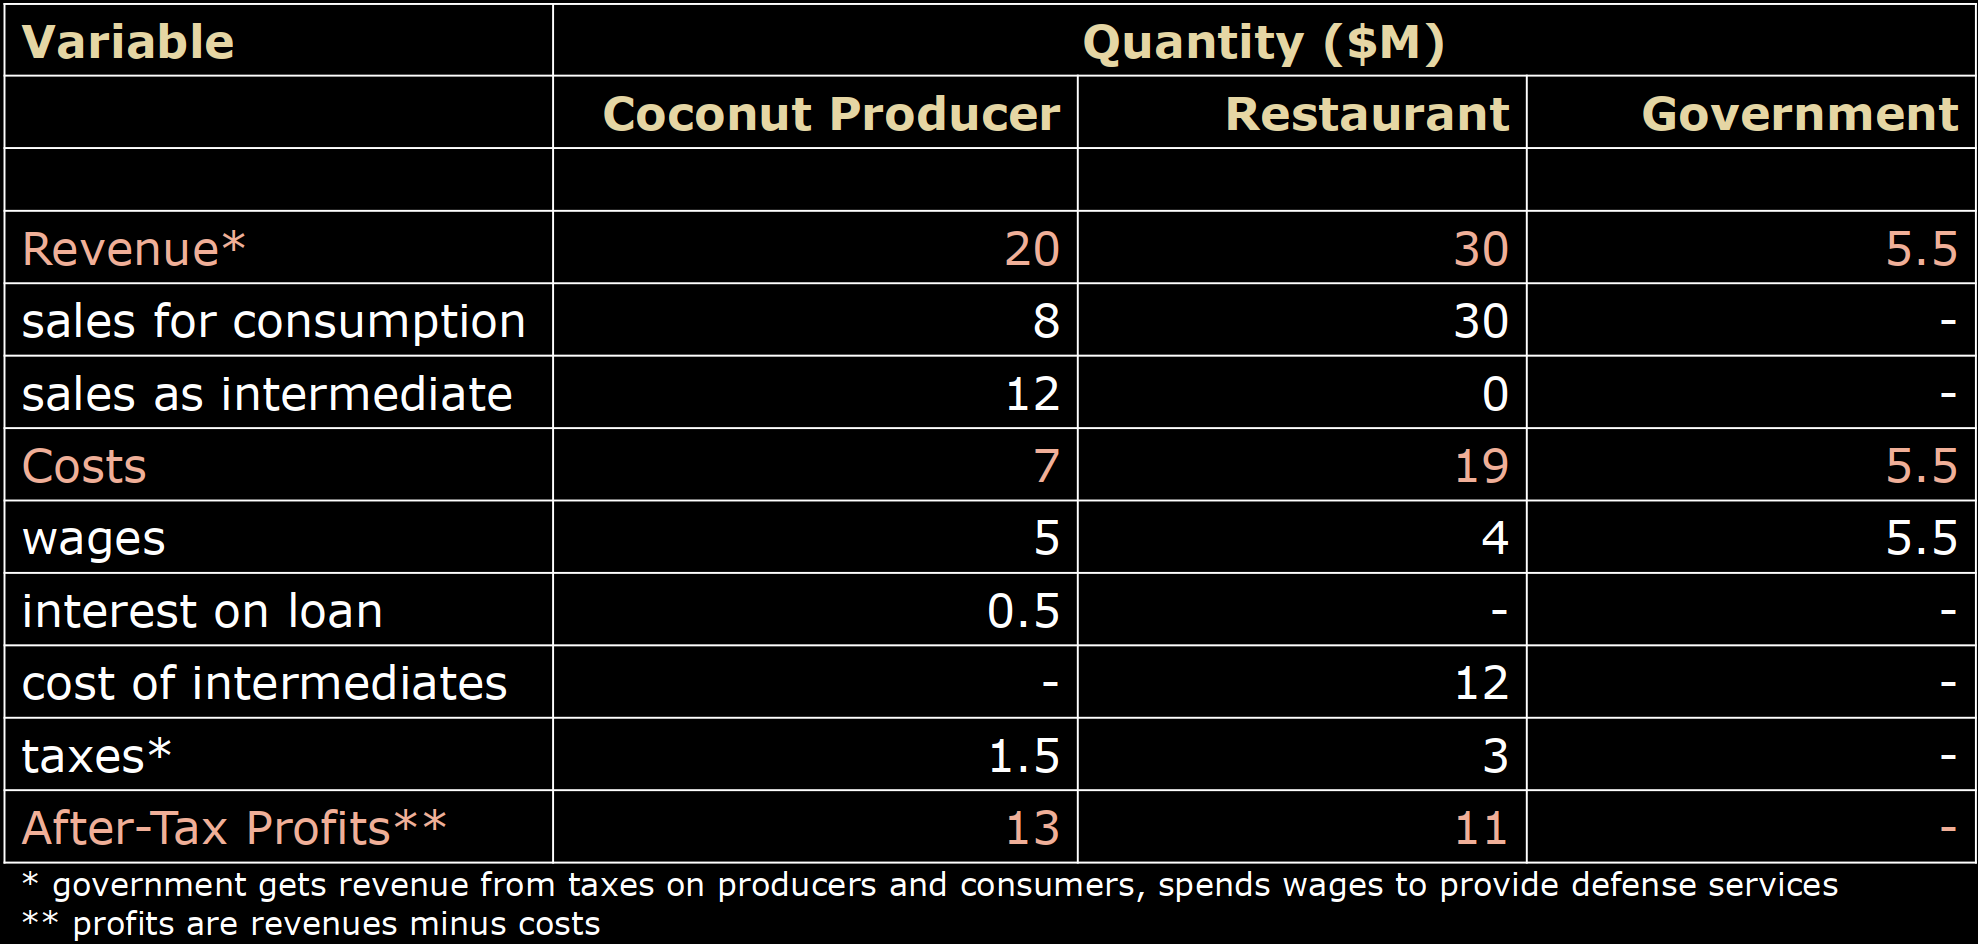
\includegraphics[width=\textwidth]{./figures/ThreeApproachTable1.png}
    % \end{figure}
\renewcommand{\arraystretch}{1.3} % row spacing
\setlength{\tabcolsep}{10pt}      % column spacing

\begin{center}
\scalebox{0.8}{
\begin{tabular}{|l|c|c|c|}
\hline
Variable & Coconut Producer & Restaurant & Government \\
\hline
\textcolor{orange}{Revenue*} & \textcolor{orange}{20} & \textcolor{orange}{30} & \textcolor{orange}{5.5} \\
\hline
sales for consumption & 8 & 30 & -- \\
sales as intermediate & 12 & 0 & -- \\
\hline
\hline
\textcolor{orange}{Costs} & \textcolor{orange}{7} & \textcolor{orange}{19} & \textcolor{orange}{5.5} \\
\hline
wages & 5 & 4 & 5.5 \\
interest on loan & 0.5 & -- & -- \\
cost of intermediates & -- & 12 & -- \\
taxes* & 1.5 & 3 & -- \\
\hline
\hline
\textcolor{orange}{After-Tax Profits**} & \textcolor{orange}{13} & \textcolor{orange}{11} & -- \\
\hline
\end{tabular}

}
\begin{minipage}{.9\textwidth}
\footnotesize
\begin{itemize}
    \item government gets revenue from taxes on producers and consumers, spends wages to provide defense services
    \item profits are revenues minus costs
\end{itemize}
\end{minipage}
\end{center}

\vspace{0.5em}

\normalsize
\alert{Question}: how to calculate GDP?
\end{frame}

\begin{frame}{The Product Approach}
\label{slide:The_Product_Approach}
\textbf{Question}: \alert{What is the value added by each agent?}

\begin{itemize}
    \item \textbf{Coconut Producer}: Final good $ \$20M $, no intermediate input
    \item \textbf{Restaurant}: Final goods $ \$30M $, with intermediate input $ \$12M $ from Coconut Producer
    \begin{itemize}
        \item value added: $ 30 - 12 = 18M $
    \end{itemize}
    \item \textbf{Government}: Defence services, valued at cost $ \$5.5M $
    \item \textbf{GDP}: $ 20 + 18 + 5.5 = 43.5M $
\end{itemize}
\end{frame}

\begin{frame}{The Expenditure Approach}
\label{slide:The_Expenditure_Approach}

\textbf{Question}: \alert{What is the total spending?}

\begin{itemize}
    \item \textbf{Formula}: $ Y = C + I + G + NX $
    \item \textbf{Consumption} ($C$): ``sale for consumption'' row
    \begin{itemize}
        \item To Coconut Producer: $ 8M $
        \item To Restaurant: $ 30M $
    \end{itemize}
    \item No investment ($ I $) and net export ($ NX $).
    \item \textbf{Government} ($G$): defense service $ 5.5M $
    \item \textbf{GDP} ($Y$): $ 38 + 5.5 = 43.5M $
\end{itemize}
\end{frame}

\begin{frame}{The Income Approach}
\label{slide:Income_Approach}
    \textbf{Question}: \alert{how much does agent earn?}
    \begin{itemize}
        \item \textbf{Workers}: wages $ 5M $ from Coconut Producer, $ 4M $ from Restaurant and $ 5.5M $ from Government
        \item \textbf{Firms}:
        \begin{itemize}
            \item After-tax Profits: $ 13M $ to Coconut Producer and $ 11M $ to Restaurant
            \item Interest on loan: $ 0.5M $ for Coconut Producer
        \end{itemize}
        \item \textbf{Government}: Taxes $ 1.5M $ from Coconut Producer and $ 3M $ from Restaurant
        \begin{itemize}
            \item Expenditure is $ 5.5M $ $ \Rightarrow  $ \alert{budget deficit}
        \end{itemize}
        \item \textbf{GDP}: $5 + 4 + 5.5 + 13 + 11 + 0.5 + 1.5 + 3 = 43.5M$
    \end{itemize}
    \textbf{Income-Expenditure Identity}: Income earned goes to expenditure
\end{frame}

\section{Inflation}
\label{sec:Inflation}

\begin{frame}{Prices in GDP measurement}
\label{slide:Prices_in_GDP_measurement}
\begin{itemize}
    \item The \alert{revenue} row is calculated by $ 10M $ coconuts $ \times $ $ \$2 $ each
    \begin{itemize}
        \item What if coconut price increases to $ \$3 $ next year?
    \end{itemize}
    \item \textbf{Solution}: common \alert{price index} across different time

    \item Two ways to build common price index:
    \begin{enumerate}
        \item GDP deflator: common \alert{GDP} standard
        \item Consumer Price Index (CPI): common \alert{consumption basket} ($Q$)
    \end{enumerate}
\end{itemize}

\end{frame}

\begin{frame}{Prices in GDP measurement (Cont.)}
\label{slide:Prices_in_GDP_measurement__Cont__}
    \begin{itemize}
        \item GDP deflator: ratio between nominal and real GDP
        \begin{enumerate}
            \item Calculate real GDP relative to base year by base year \alert{price level}
            \begin{itemize}
                \item E.g. $ RealGDP_{2020} = \text{Cost of } Q_{2020} \text{ at } P_{\alert{2000}} $, use $ 2000 $ as base year
                \item While $ NominalGDP_{2020} = \text{Cost of } Q_{2020} \text{ at } P_{\alert{2020}} $
                \item \alert{Problem}: choose which year? $ \Rightarrow  $ ``\alert{chain-weighting}'' (rolling base)
            \end{itemize}
            \item Calculate ratio: $ \frac{NominalGDP_{2020}}{RealGDP_{2020}} \times 100 $
        \end{enumerate}
        \item CPI: normalize \alert{consumption basket} of \alert{base year} as $ 100 $, relative to \alert{other year}
        \begin{itemize}
            \item E.g. $ CPI_{2020} = \frac{\text{Cost of } Q_{2000} \text{ at } P_{2020}}{\text{Cost of } Q_{2000} \text{ at } P_{2000}} \times 100 $, use $ 2000 $ as base year
            \item \alert{Problem}:
            \begin{enumerate}
                \item $ \Delta P $ outside of consumption basket \&  not accounted
                \item new goods \& services introduced, old goods \& services obsolete
            \end{enumerate}
        \end{itemize}
    \end{itemize}
\end{frame}

\begin{frame}{Example: Nominal v.s. Real GDP}
\label{slide:Example__Nominal_v_s__Real_GDP}
    \begin{itemize}
        \item \textbf{Nominal GDP}: value of goods \& services at current price
        \item \textbf{Real GDP}: value of goods \& services at base year price
    \end{itemize}
\begin{center}
\scalebox{0.9}{
\begin{tabular}{|c|c|c|c|c|c|c|c|}
\hline
\multicolumn{1}{|c|}{\bfseries Year} &
\multicolumn{2}{c|}{\bfseries Apples} &
\multicolumn{2}{c|}{\bfseries Oranges} &
\multicolumn{3}{c|}{\bfseries GDP Measure} \\
\hline
 & Quantity & Price & Quantity & Price & Nominal & Real (base year = 1) & Real (base year = 2) \\
\hline
1 & 50 & \$1.00 & 100 & \$0.80 & \$130 & \$130 & \$222.5 \\
2 & 80 & \$1.25 & 120 & \$1.60 & \$292 & \$176 & \$292 \\
\hline
\end{tabular}}
\end{center}
\begin{itemize}
    \item Choice of base year affects the GDP measure!
    \item Alternative: chain-weighting
\end{itemize}

\end{frame}

\begin{frame}{Data: Nominal v.s. Real GDP}
\label{slide:Data__Nominal_v_s__Real_GDP}
    \begin{columns}
        \begin{column}{0.4\textwidth}
            \begin{itemize}
                \item inflation growth $ + $ economics growth $ = $ nominal grows faster than real
                \item \textbf{Question}: \alert{What year is the base year} on this graph?
                \item Ans: 2009, when Nominal $ = $ Real
            \end{itemize}
        \end{column}
        \begin{column}{0.6\textwidth}
            \begin{figure}
                \caption{Figure 2.1 Nominal GDP and Chain-Weighted Real GDP}
                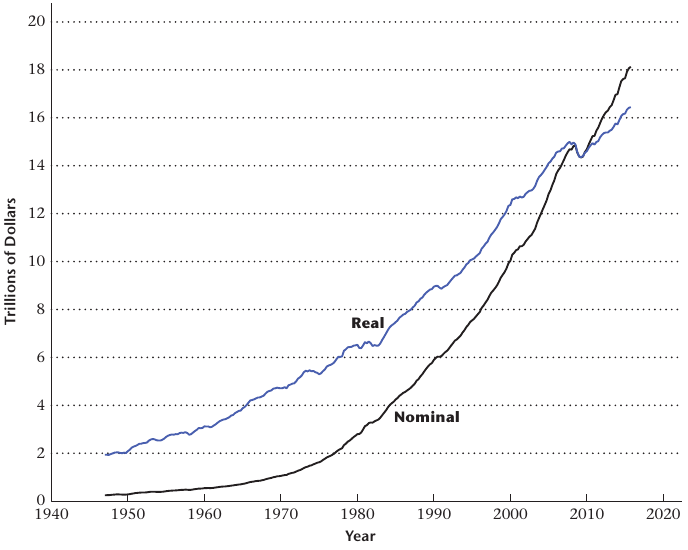
\includegraphics[width=.9\textwidth]{./figures/Figure2_1.png}
            \end{figure}
        \end{column}
    \end{columns}
\end{frame}

\section{Employment}
\label{sec:Employment}

\begin{frame}{Population Composition}
\label{slide:Population_Composition}
    \hspace{11em} N \hspace{7em} LF \hspace{5em} E/U
    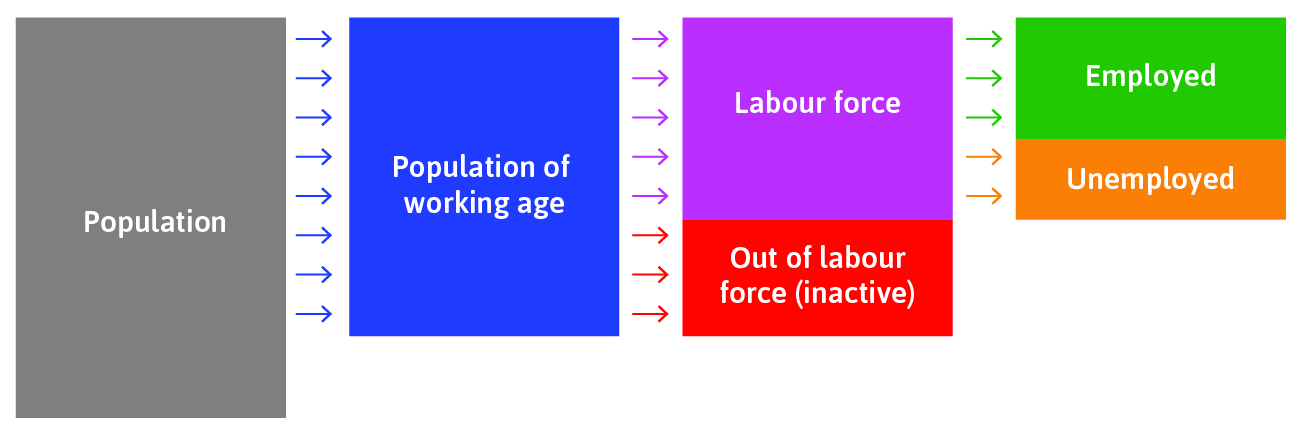
\includegraphics[width=\textwidth]{./figures/employmentPop.jpg}
    \begin{itemize}
        \item participation rate $ = \frac{LF}{N} $
        \item unemployment rate $ = \frac{U}{\alert{LF}} $
        \item employment rate $ = \frac{E}{\alert{N}} $
    \end{itemize}
\end{frame}

% \appendix

% \begin{frame}[allowframebreaks]{References}
% \footnotesize
% \bibliographystyle{$BIB_STYLE}
% \bibliography{$BIBFILE}
% \end{frame}

\end{document}



\end{document}

